%%%%%%%%%%%%%%%%%%%%%%%%%%%%%%%%%%%%%%%%%%%%%%%%%%%%%%%%%%%%%%%%%%%%%%%%%%%%%%%%%%%%%%%%%%
%%% QUESTA SEZIONE CONTIENE FRASI TIRATE VIA DA ALTRI CAPITOLI
%%%%%%%%%%%%%%%%%%%%%%%%%%%%%%%%%%%%%%%%%%%%%%%%%%%%%%%%%%%%%%%%%%%%%%%%%%%%%%%%%%%%%%%%%%

% \section{Alternative approaches to Modularity}
% If the problems of Modularity are evident, researchers tried to mitigate them with alternative meta-approaches. The issue of degeneracy indeed, implicitly maintains that in the absence of a clearly optimal partition, many partitions should be used instead. Yet, the problem of the resolution limit that arises from an inadequate choice of the configuration model as the null hypothesis, can be tackled by a proper choice of the null model that keeps into account the sources of random noise directly from the time series which the correlation matrix is originated from. Here we briefly discuss these two potential solutions to the problems we have just introduced.

% \subsection{The bias of the null model for Modularity}
% The null model of Modularity is not only is at the basis of the issues of resolution limit and degeneracy, but can be shown to be highly inadequate when used in brain networks based on estimates of Pearson correlation of BOLD time series.
% As shown by MacMahon and Garlaschelli~\cite{macmahon2015}, indeed the configuration model introduces a systematic bias as it is not consistent with the definition of Pearson correlation.
% Ideally, the modular structure in a full correlation matrix (a correlation matrix with all nonzero entries) should reflect a balance between positively and negatively correlated units. Correlation communities should be internally positively correlated while externally negatively correlated, but this does not happen when naively applying Modularity to correlation-based networks.
% Such inadequacy results from a systematic bias that the configuration model introduces, here shortly explained.

% Given $n$ time series $\mathbf{X}=\{ X_1, \ldots, X_n\}$ from the parcellation atlas, the Pearson correlation matrix is computed as
% \begin{equation}
% C_{ij} = \frac{\textrm{Cov}(X_i,X_j)}{\sqrt{\textrm{Var}(X_i)\textrm{Var}(X_j) }}.
% \end{equation}
% A naive application of Newman's Modularity to such correlation matrix results in:
% \begin{equation}
% Q^N= \frac{1}{C_{\textrm{norm}}} \sum \limits_{ij} \left[ C_{ij} - \langle C_{ij} \rangle \right] \delta(\sigma_i,\sigma_j) = \left[ C_{ij} - \frac{k_i k_j}{C_{\textrm{norm}}} \right] \delta(\sigma_i,\sigma_j)
% \end{equation}
% where $k_i=\sum_{j=1}^n C_{ij}$. Unfortunately though, this last term is biased because expanding the terms $k_i$ one obtains:
% \begin{equation}
% k_i =\sum_{j=1}^n C_{ij}= \sum_{j=1}^n \textrm{Cov}(X_i,X_j) = \sum_{j=1}^n \textrm{Cov}(X_i,X_{tot})
% \end{equation}
% where $X_{tot}=\sum_{j=1}^n x_j$ has zero mean but non unit variance, and the configuration model naively applied to correlation matrices becomes:
% \begin{equation}
% \frac{k_i k_j}{2m} = \textrm{Corr}(X_i,X_{tot})\textrm{Corr}(X_j,X_{tot})
% \end{equation}
% Such badly-adapted configuration model does not give more importance to pairs of strongly correlated time series but rather to pairs of time series whose direct correlation $C_{ij}$ is larger than the common signal $X_{tot}$.
% The null model proposed by MacMahon and Garlaschelli redefines the null model of Modularity to take into consideration such desired property. Thanks to the \emph{random matrix theory} the bulk of signal due to the global mode, a large-scale oscillation that positively correlates all areas, is removed and only terms that retain true correlations are maintained.

%\todo{questo calcolo è sbagliato perchè considera } In fact, the number of possible sequences of node labels with prescribed degree sequence that can be generated under the hypotheses of the configuration model, namely the presence of self-loops and multi-edges, is indicated by $\Omega_{CM}$ and can be computed by means of combinatorial arguments as the multinomial distribution:
% \begin{equation}\label{eq:cm_possible_rewirings}
% \Omega_{CM} = \binom{2m}{k_1,\ldots,k_n} = \frac{(2m)!}{\prod_i^n k_i!}.
% \end{equation}
% For the small triangle graph, this number is already very large: 90 different re-wirings are possible!


% % Unfortunately, until recently most of the studies in animal models were based on anatomical connectivity measured by means of post-mortem inspections.
% % While in the past, histological staining was the most adopted methodology to inspect the wiring of white matter in the animal brain, the last few decades have seen the rising of fluorescence based tract-tracing, that evolved to a level where single axons can be traced with unprecedented precision~\cite{oh2014}.
% % Not only methods to investigate the structural connectivity have greatly evolved, but also new cellular resolution recording systems, like light-sheet microscopy~\cite{ahrens2013}, real time in-vivo two-photon cortical imaging~\cite{dombeck2010,leinweber2014} and spike time series recordings on multielectrode arrays~\cite{shimono2015}.
% % All these techniques take part in the quest to shed light on the relation between functional networks and their underlying anatomical substrate.

% After the discovery of low frequency fluctuations of the BOLD signal of the brain at rest~\cite{biswal1995}, 
% In humans, non-invasive studies of the brain community structure largely reflect the analytical methodologies adopted in animals.
% In both contexts, functional connectivity is suggested to describe the relationship between neuronal activity patterns of anatomically separated regions that reflect the level of information exchange between them.
% The decomposition of the endogenous fluctuations of the BOLD signal at rest by means of independent components analysis (ICA), showed a repertoire of \emph{spatial modes}, clusters of brain regions whose neural activity oscillates synchronously. These patterns of spontaneous coupled oscillations are strongly correlated between anatomically separated, possibly remote regions of the brain~\cite{biswal1995,raichle2001,fox2005,biswal2012}. Additionally, these patterns of functional connections that derive from a modular architecture of the brain, are themselves modular. A submodule (or subnetwork), often called community in graph theory, comprises synchronously active voxels. The enduring and stable synchrony within those voxels is thought to reflect local integration processes



% The evidence of modules in functional brain networks has been explained as the possible basis of a large variety of processes. By way of example, certain functional processes, like color vision, have been described as anatomically localized~\cite{zeki1998}, while others, like working memory, have been proposed to involve more globally integrated processing systems~\cite{dehaene1998,baddeley2003}.
% Interestingly modules of functional brain networks are non-static as recent studies found that they tend to become less and less modular with aging~\cite{meunier2009a,song2014}. 
% In all respects, the experimental evidence of the modular organization is a powerful and robust marker against which to measure the health of the brain. 
% Thus, modularity is not only a biologically plausible feature but it is probably necessary to maintain the rich repertoire of cognitive tasks that our brain engages in every day of our life.

% Despite the biological evidence of modularity in brain networks, the number of modules returned by clustering methods is often chosen in advance, based on the experience of the researcher, even if some complex approaches are available~\cite{still2004}. 


%%%%%%%%%%%%%% CAPITOLO 5 SCHIZOFRENIA %%%%%%%%%%
% The ability to resolve these changes at a finer scale than previously possible sheds new light on the functional implications of aberrant functional connectivity in Schizophrenia.
% \section{Functional connectivity parameters in Schizophrenia patients and healthy controls}
% To examine the difference in functional connectivity between the two populations, I computed group-level graphs, each consisting of 638 nodes fully connected by edges reflecting Pearson pairwise correlations between resting state fluctuations of the BOLD signals.
% \begin{figure}
% \centering
% 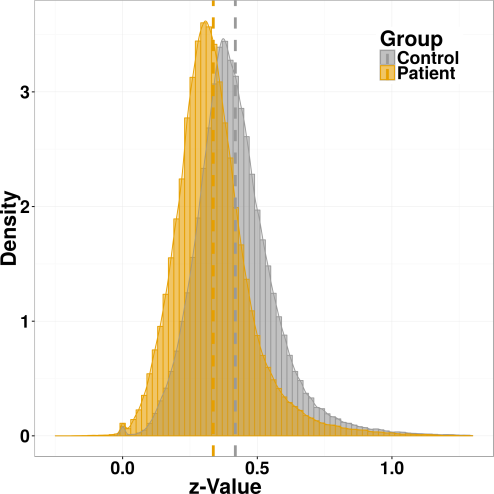
\includegraphics[width=1.0\textwidth]{images/schizo/schizo_fig_1.png}
% \caption{$z$-value distribution of the adjacency matrix for both populations.}
% \label{fig:ttest_schizo}
% \end{figure}
% Figure~\ref{fig:ttest_schizo} shows the edge-weight distribution for the two groups.
% We observed a significant shift in the average z-score value of the matrix between the patient and the control (t-test $p\textrm{value} < 10^{-16}$).
% \begin{figure}
% \centering
% 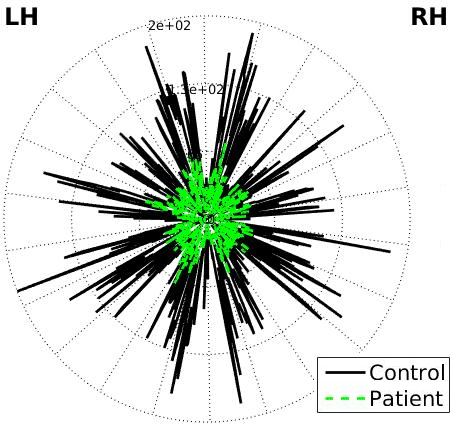
\includegraphics[width=0.4\textwidth]{images/schizo/schizo_fig_2a.jpg}
% 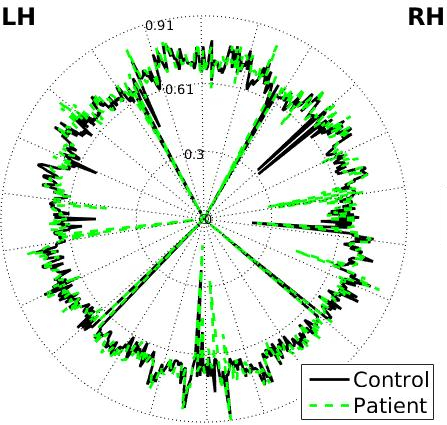
\includegraphics[width=0.4\textwidth]{images/schizo/schizo_fig_2b.jpg}
% \caption{A. Degree of each nodes; B. Local efficiency value by nodes. The nodes of the left and on the right hemisphere are respectively on the right and on the left of the circle.}
% \label{fig:schizo_degree}
% \end{figure}
% Figure~\ref{fig:schizo_degree} shows the distribution of node degree, a node-wise parameter that measures the number and strength of edges incident to each node.
% A significant decrease of average node-degree was observed for the SCZ groups (green line) compared to the CON group (black line), with degree values of $25.73 \pm 13.04$ and $53.83 \pm 40.35$ respectively \todo{Statistical significance?}.
% Additionally, we computed the global efficiency coefficient $E(G)$, i.e.
% the inverse average path length connecting any two nodes, a measure of how efficiently information is exchanged across the network.
% $E(G)$ was strongly reduced in the SZ group, with a value of $0.23$ versus $0.32$ for the control group, a further indication of reduced network integration in the patient.
% Altogether, these analyses show reduction in functional connectivity in the Schizophrenia group, entirely consistent with previous reports~\cite{liu2008,alexander-bloch2010,lerman-sinkoff2016}.
% Interestingly, though, local efficiency, defined as the efficiency of a node's local network of nearest neighbors when the node is removed, was similar for the two groups (Control= $0.67\pm0.09$, Patient= $0.68\pm0.09$).
% Figure~\ref{fig:schizo_degree}B shows local efficiency for each node, with green and black lines denoting patients and controls, respectively.
% The graph reveals only minor differences between the two populations, thus suggesting that network tolerance to node faults is generally preserved or even improved in patients compared to controls even if functional connectivity is substantially weaker~\cite{lynall2010}.
% This has been observed in previous studies, and pointed to as a potential evolutionary advantage that may justify persistence of schizophrenia-related genes in the general population~\cite{lynall2010}, but its implications remain speculative.
% In summary, all graph-related parameters measured in this study appear consistent with those reported in the literature for smaller groups or specific sub-populations of patients (e.g. childhood onset schizophrenics), thus corroborating the idea that the present data-set has global and node-wise functional connectivity features that are comparable to those of previous studies.
% In the following, we investigate the effects of these scale-dependent differences in functional connectivity on the modular organization of functional connectivity in schizophrenia patients vs controls.